\documentclass[../main.tex]{subfiles}

\begin{document}
Projekt wykorzystuje bazę danych do przechowywania i zarządzania danymi filmów, recenzji, komentarzy, użytkowników, oraz dodatkowych szczegółów takich jak reżyserzy, obsada, i gatunki.

\subsection{Logiczny model danych}
Na rysunku \ref{fig:model_danych:logiczny} zaprezentowany został logiczny model danych (schemat ERD) używanej bazy danych.
\begin{figure}[htb]
	\centering
	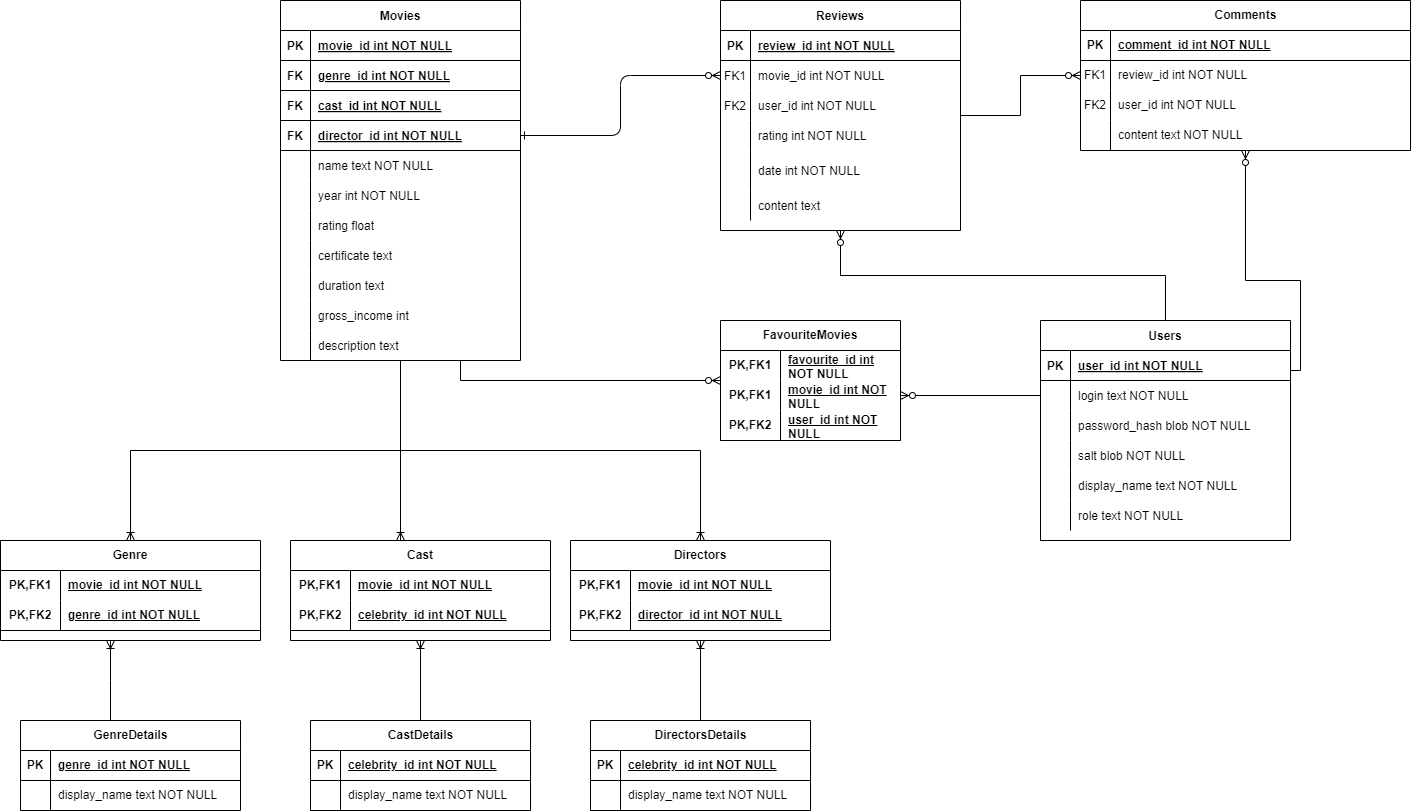
\includegraphics[width=0.9\textwidth]{model_danych/logiczny_model_danych.png}
	\caption{Logiczny model danych}
	\label{fig:model_danych:logiczny}
\end{figure}

\subsection{Fizyczny model danych}
Do realizacji modelu danych użyty został silnik bazodanowy PostgreSQL. Schemat fizyczny bazy danych widoczny jest na rysunku \ref{fig:model_danych:fizyczny}.

\begin{figure}[htb]
	\centering
	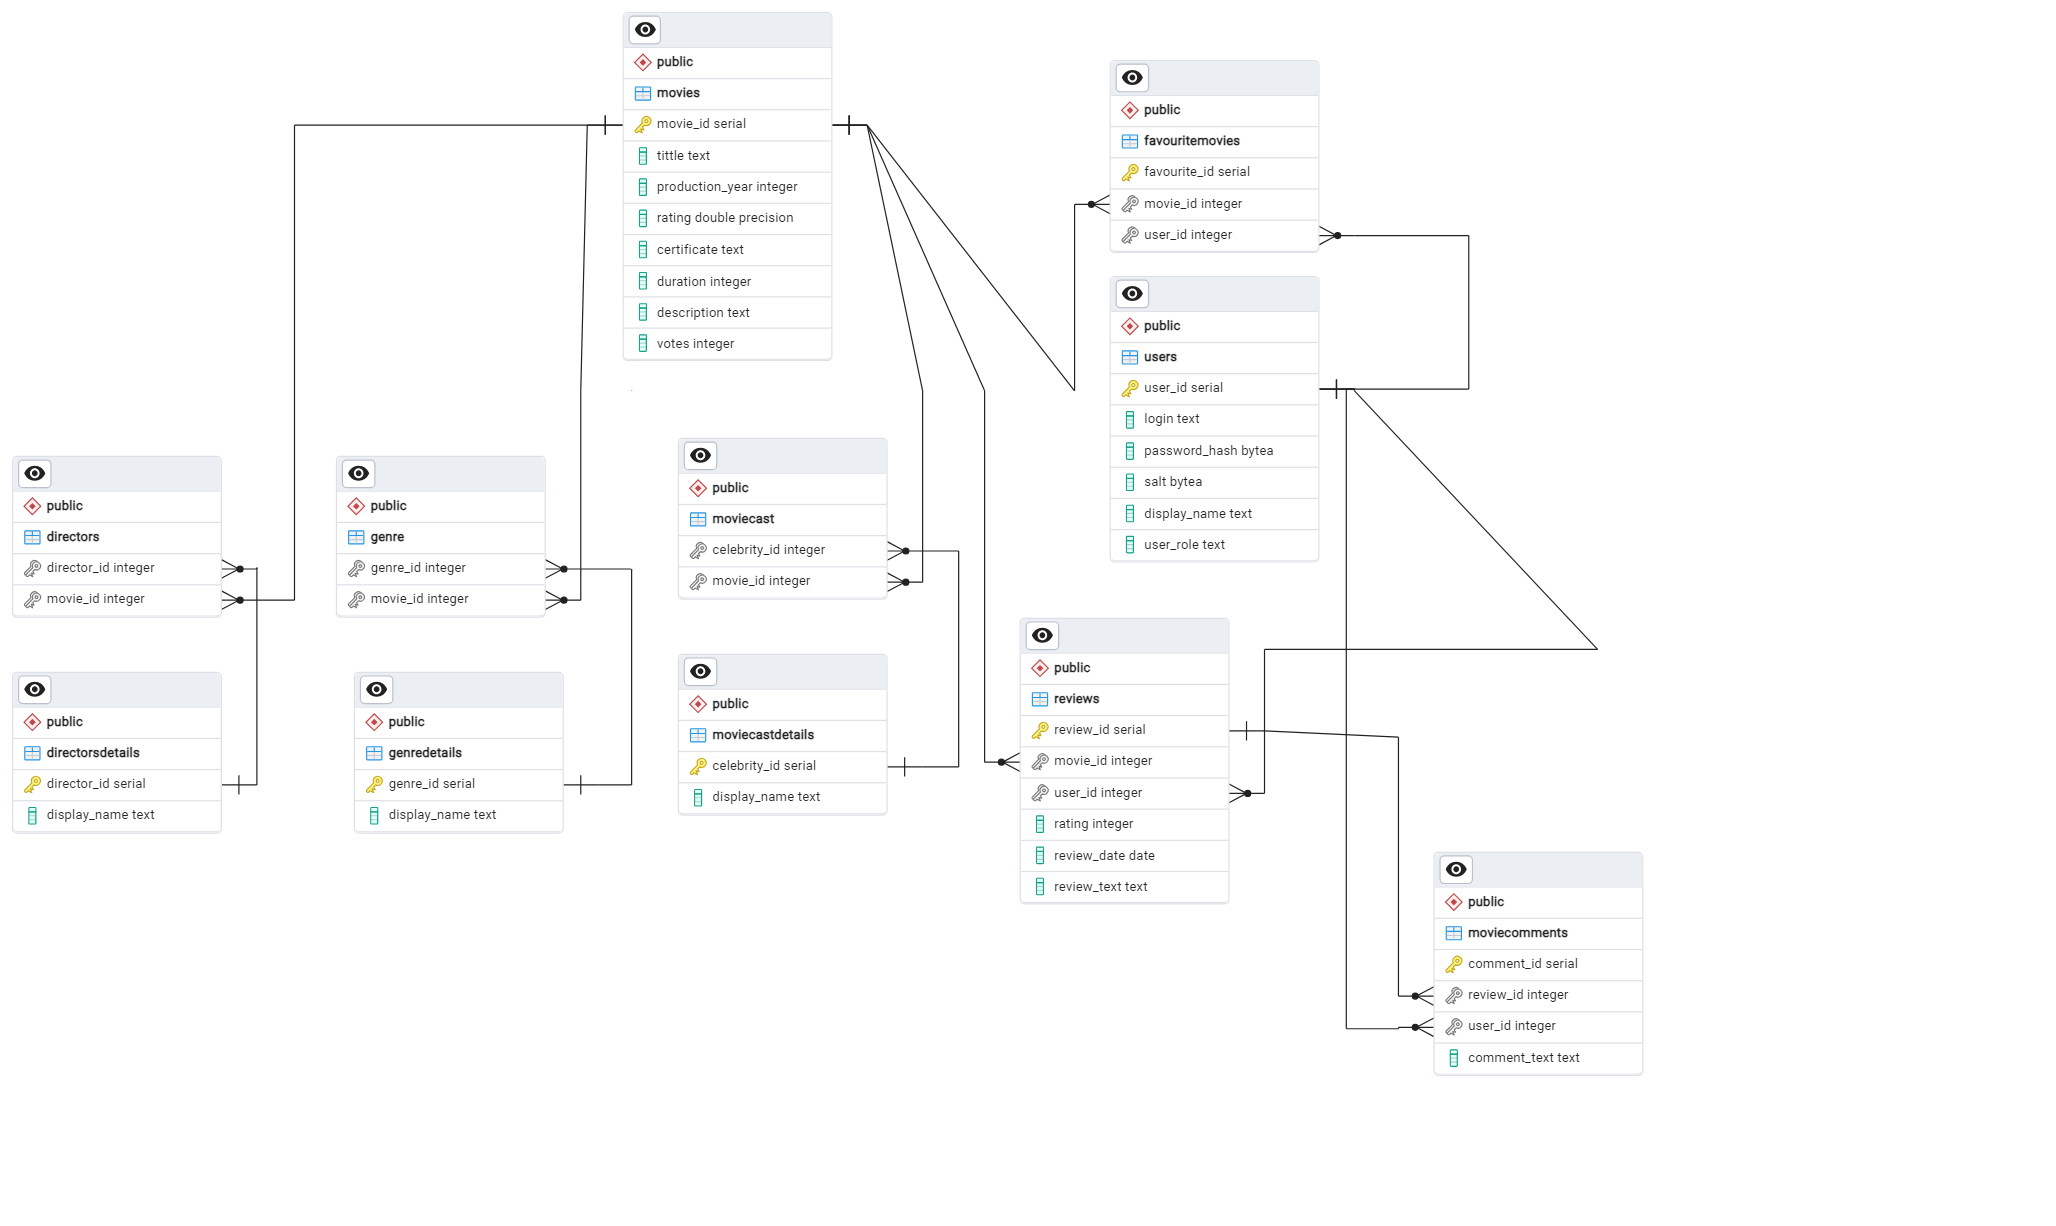
\includegraphics[width=0.9\textwidth]{model_danych/fizyczny_model_danych.png}
	\caption{Fizyczny model danych}
	\label{fig:model_danych:fizyczny}
\end{figure}

\subsection{Dokładne opisy tabel}
Poniżej znajduje się dokładny opis każdej z tabel:
\begin{itemize}
	\item \texttt{Movies}: zawiera informacje o filmach
	      \begin{itemize}
		      \item \texttt{movie\_id}: klucz główny, numer identyfikacyjny filmu.
		      \item \texttt{title}: tytuł filmu.
		      \item \texttt{production\_year}: rok produkcji filmu.
		      \item \texttt{rating}: ocena filmu.
		      \item \texttt{certificate}: certyfikat filmu (np. PG-13).
		      \item \texttt{duration}: czas trwania filmu w minutach.
		      \item \texttt{description}: opis filmu.
		      \item \texttt{votes}: liczba głosów oddanych na film.
	      \end{itemize}
	\item \texttt{Reviews}: zawiera informacje o recenzjach
	      \begin{itemize}
		      \item \texttt{review\_id}: klucz główny, numer identyfikacyjny recenzji.
		      \item \texttt{movie\_id}: klucz obcy, odnosi się do tabeli Movies.
		      \item \texttt{user\_id}: klucz obcy, odnosi się do tabeli Users.
		      \item \texttt{rating}: ocena przyznana w recenzji.
		      \item \texttt{review\_date}: data wystawienia recenzji.
		      \item \texttt{review\_text}: treść recenzji.
	      \end{itemize}
	\item \texttt{Users}: zawiera informacje o użytkownikach
	      \begin{itemize}
		      \item \texttt{user\_id}: klucz główny, numer identyfikacyjny użytkownika.
		      \item \texttt{login}: login użytkownika.
		      \item \texttt{password\_hash}: zahaszowane hasło użytkownika.
		      \item \texttt{salt}: sól do hashowania hasła.
		      \item \texttt{display\_name}: wyświetlana nazwa użytkownika.
		      \item \texttt{user\_role}: rola użytkownika w systemie (np. admin, standardowy użytkownik).
	      \end{itemize}
	\item \texttt{MovieComments}: zawiera informacje o komentarzach do filmów
	      \begin{itemize}
		      \item \texttt{comment\_id}: klucz główny, numer identyfikacyjny komentarza.
		      \item \texttt{review\_id}: klucz obcy, odnosi się do tabeli Reviews.
		      \item \texttt{user\_id}: klucz obcy, odnosi się do tabeli Users.
		      \item \texttt{comment\_text}: treść komentarza.
	      \end{itemize}
	\item \texttt{FavoriteMovies}: zawiera informacje o ulubionych filmach użytkowników
	      \begin{itemize}
		      \item \texttt{favourite\_id}: klucz główny, numer identyfikacyjny ulubionego filmu.
		      \item \texttt{movie\_id}: klucz obcy, odnosi się do tabeli Movies.
		      \item \texttt{user\_id}: klucz obcy, odnosi się do tabeli Users.
	      \end{itemize}
	\item \texttt{DirectorsDetails}: zawiera informacje o reżyserach
	      \begin{itemize}
		      \item \texttt{director\_id}: klucz główny, numer identyfikacyjny reżysera.
		      \item \texttt{display\_name}: nazwa wyświetlana reżysera.
	      \end{itemize}
	\item \texttt{Directors}: tworzy relację między reżyserami oraz filmami, które wyreżyserowali
	      \begin{itemize}
		      \item \texttt{director\_id}: klucz obcy, odnosi się do tabeli DirectorsDetails.
		      \item \texttt{movie\_id}: klucz obcy, odnosi się do tabeli Movies.
	      \end{itemize}
	\item \texttt{MovieCastDetails}: zawiera informacje o roli danej osoby w filmie
	      \begin{itemize}
		      \item \texttt{celebrity\_id}: klucz główny, numer identyfikacyjny osoby z obsady.
		      \item \texttt{display\_name}: nazwa wyświetlana osoby z obsady.
	      \end{itemize}
	\item \texttt{MovieCast}: tworzy relację między celebrytami a filmami, w których grali
	      \begin{itemize}
		      \item \texttt{celebrity\_id}: klucz obcy, odnosi się do tabeli MovieCastDetails.
		      \item \texttt{movie\_id}: klucz obcy, odnosi się do tabeli Movies.
	      \end{itemize}
	\item \texttt{GenreDetails}: zawiera informacje o gatunkach filmów
	      \begin{itemize}
		      \item \texttt{genre\_id}: klucz główny, numer identyfikacyjny gatunku.
		      \item \texttt{display\_name}: nazwa wyświetlana gatunku.
	      \end{itemize}
	\item \texttt{Genre}: tworzy relację między filmem a jego gatunkiem
	      \begin{itemize}
		      \item \texttt{genre\_id}: klucz obcy, odnosi się do tabeli GenreDetails.
		      \item \texttt{movie\_id}: klucz obcy, odnosi się do tabeli Movies.
	      \end{itemize}
\end{itemize}

\subsection{Relacje}
\begin{itemize}
	\item \texttt{Movies}-\texttt{GenreDetails} (wiele-do-wielu) - tabela \texttt{Genres}. Tabela ta zarządza relacjami między filmami a gatunkami, umożliwiając przypisanie wielu gatunków do jednego filmu i odwrotnie. Jest to typowa relacja wiele-do-wielu realizowana przez tabelę łączącą zawierającą klucze obce odnoszące się zarówno do \texttt{Movies} jak i \texttt{GenreDetails}.
	\item \texttt{Movies}-\texttt{DirectorsDetails} (wiele-do-wielu) - tabela \texttt{Directors}: Podobnie jak w przypadku gatunków, ta tabela łącząca zarządza relacją między filmami a reżyserami, umożliwiając przypisanie wielu reżyserów do jednego filmu (często w przypadku współreżyserii) oraz przypisanie jednego reżysera do wielu filmów. Każdy rekord łączy film z reżyserem za pomocą kluczy obcych wskazujących na \texttt{Movies} i \texttt{DirectorsDetails}.
	\item \texttt{Movies}-\texttt{MovieCastDetails} (wiele-do-wielu) - tabela \texttt{MovieCast}. Ta tabela służy jako mostek dla relacji wiele-do-wielu między filmami a ich obsadą. Umożliwia to, że jeden film może mieć wielu członków obsady i odwrotnie, korzystając z kluczy obcych wskazujących na \texttt{Movies} i \texttt{MovieCastDetails}.
	\item \texttt{Movies}-\texttt{Users} (jeden-do-wielu) - tabela \texttt{Reviews}. Tabela \texttt{Reviews} przechowuje recenzje, które użytkownicy piszą o filmach. Każda recenzja jest powiązana z dokładnie jednym filmem i jednym użytkownikiem, co przedstawia relację jeden-do-wielu od \texttt{Movies} do \texttt{Reviews} (jeden film może mieć wiele recenzji) oraz od \texttt{Users} do \texttt{Reviews} (jeden użytkownik może napisać wiele recenzji)/
	\item \texttt{Movies}-\texttt{Users} (jeden-do-wielu) - tabela \texttt{MovieComments}. Każdy komentarz w tabeli \texttt{MovieComments} jest powiązany z dokładnie jedną recenzją i jednym użytkownikiem. Ta konfiguracja tworzy relację jeden-do-wielu od \texttt{Reviews} do \texttt{MovieComments} (jedna recenzja może mieć wiele komentarzy) oraz od \texttt{Users} do \texttt{MovieComments} (jeden użytkownik może zamieścić wiele komentarzy).
	\item \texttt{Movies}-\texttt{Users} (wiele-do-wielu) - tabela \texttt{FavoriteMovies}. Tabela \texttt{FavouriteMovies} śledzi, którzy użytkownicy dodali które filmy do ulubionych. Choć funkcjonuje to jako relacja wiele-do-wielu (użytkownik może mieć wielu ulubionych filmów i film może być ulubiony przez wielu użytkowników), jest reprezentowane bez typowej tabeli łączącej, ponieważ każdy rekord w \texttt{FavouriteMovies} niejako reprezentuje link między użytkownikiem a filmem.
\end{itemize}

\subsection{Skrypty SQL}
Tabele oraz relacje między nimi zostały stworzone przy użyciu skryptów SQL zamieszczonych w tabelach \ref{tab:model_danych:skrypty_sql} oraz \ref{tab:model_danych:relacje_sql}.

\newcommand{\quicksql}[1]{
	\begin{minipage}[t]{0.49\textwidth}
		\centering
		\inputminted[fontsize=\footnotesize]{sql}{./resources/code/model_danych/#1}
	\end{minipage}
}
\newcommand{\newhline}{\\\hline}

\begin{table}[htb]
	\caption{Skrypty SQL tworzące poszczególne tabele}
	\label{tab:model_danych:skrypty_sql}

	\begin{tabular}{| p{0.49\textwidth} | p{0.49\textwidth} |}
		\hline
		\quicksql{movies.sql}          & \quicksql{reviews.sql} \newhline
		\quicksql{users.sql}           & \quicksql{moviecomments.sql} \newhline
		\quicksql{favouritemovies.sql} & \quicksql{directorsdetails.sql} \newhline
		\quicksql{directors.sql}       & \quicksql{moviecastdetails.sql} \newhline
		\quicksql{moviecast.sql}       & \quicksql{genredetails.sql} \newhline
		\quicksql{genre.sql}           & \newhline
	\end{tabular}
\end{table}



\begin{table}[htb]
	\caption{Skrypty SQL tworzące relacje między poszczególnymi tabelami}
	\label{tab:model_danych:relacje_sql}

	\begin{tabular}{| p{0.99\textwidth} |}
		\hline
		\quicksql{alter_moviecast.sql} \newhline
		\quicksql{alter_directors.sql} \newhline
		\quicksql{alter_genre.sql} \newhline
		\quicksql{alter_reviews.sql} \newhline
		\quicksql{alter_moviecomments.sql} \newhline
		\quicksql{alter_favouritemovies.sql} \newhline
	\end{tabular}
\end{table}

\subsection{Przykładowy zestaw danych}
Otrzymany zestaw danych nie jest podzielony odpowiednio pod utworzone tabele. Z wykorzystaniem kilku prostych programów napisanych w Pythonie z użyciem biblioteki \texttt{pandas}, udało nam się przetworzyć oraz przetransformować dane w odpowiedni sposób. \texttt{Python}, ze swoją wszechstronnością i obszernym ekosystemem bibliotek takich jak pandas, jest idealnym narzędziem do manipulacji danymi, szczególnie w przypadkach, gdy wymagana jest elastyczność w przetwarzaniu i transformacji zestawów danych. 
Przykładowe zestawy danych po obróbce można znaleźć na rysunku \ref{fig:model_danych:dane}.

\begin{figure}[htb]
	\centering

	\begin{subfigure}{1\textwidth}
		\centering
		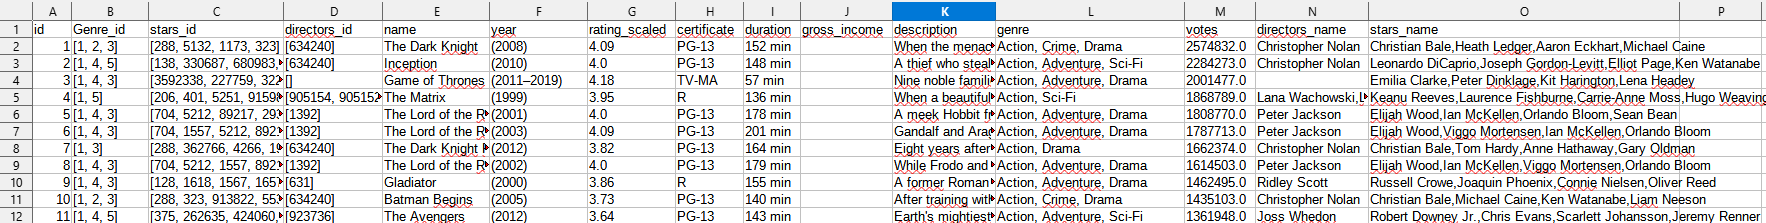
\includegraphics[width=\textwidth]{model_danych/csv_input.png}
		\caption{Surowe dane wejściowe}
		\label{fig:model_danych:csvin}
	\end{subfigure}
	\hrule
	\begin{subfigure}{0.27\textwidth}
		\vspace{\baselineskip}
		\centering
		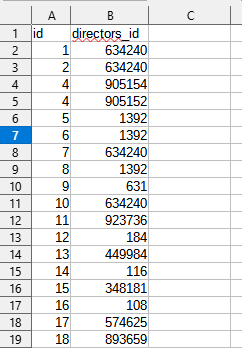
\includegraphics[width=0.95\textwidth]{model_danych/csv_directors.png}
		\caption{Dane do tabeli \texttt{Directors}}
		\label{fig:model_danych:csvdirectors}
	\end{subfigure}
	\vertline
	\begin{subfigure}{0.4\textwidth}
		\vspace{\baselineskip}
		\centering
		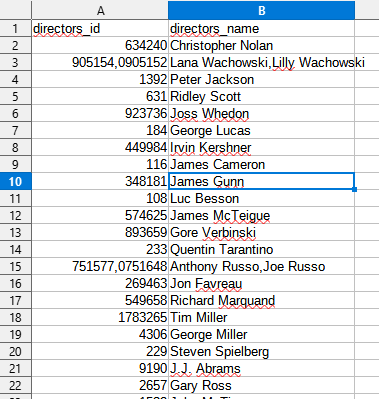
\includegraphics[width=0.95\textwidth]{model_danych/csv_directors_details.png}
		\caption{Dane do tabeli \texttt{DirectorsDetails}}
		\label{fig:model_danych:csvdirectorsdetails}
	\end{subfigure}
	\vertline
	\begin{subfigure}{0.27\textwidth}
		\vspace{\baselineskip}
		\centering
		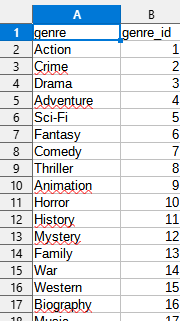
\includegraphics[width=0.95\textwidth]{model_danych/csv_genre.png}
		\caption{Dane do tabeli \texttt{Genre}}
		\label{fig:model_danych:csvgenres}
	\end{subfigure}

	\caption{Przykładowe dane wejściowe (\subref{fig:model_danych:csvin}) oraz ich transformacje (\subref{fig:model_danych:csvdirectors}-\subref{fig:model_danych:csvgenres})}
	\label{fig:model_danych:dane}

\end{figure}

\end{document}